\documentclass[fleqn,10pt]{wlscirep}

% --- Packages ---
\usepackage{graphicx}
\usepackage{caption}
\usepackage{subcaption}
\usepackage{float}
\usepackage{amsmath}
\usepackage{amssymb}
\usepackage{hyperref}

% --- Graphics path (adjust to your repo layout) ---
\graphicspath{{NHB_Symbolic_Mainfold/code/figs_final/}{./}}

% --- Captions ---
\captionsetup{labelfont=bf,font=small}

% --- Raster formats ---
\DeclareGraphicsExtensions{.pdf,.png,.jpg}

\title{Symbolic Manifolds and Entropic Dynamics: A Computational Framework for Monitoring Cognitive Network Recovery in Regenerative Medicine}

\author[1]{Demetrios Agourakis}
\author[1]{Dionisio Chiuratto Agourakis}
\author[2]{Renata Rigacci Abdala}
\author[3]{Marina Stahl Merlin}
\author[4]{Marli Gerenutti}

\affil[1]{[Institution of Demetrios and Dionisio], [City], [Country]}
\affil[2]{[Institution of Dr.\ Renata Rigacci Abdala], [City], [Country]}
\affil[3]{[Institution of Marina Stahl Merlin], [City], [Country]}
\affil[4]{[Institution of Dr.\ Marli Gerenutti], [City], [Country]}

\affil[*]{Corresponding author: demetrios@agourakis.med.br}

\begin{abstract}
Cognitive recovery requires more than structural repair: it depends on the re-emergence of symbolic--semantic organisation. We present an open framework that projects large-scale semantic associations (SWOW-EN) onto a \emph{symbolic manifold} where network topology, entropy-controlled exploration and discrete curvature jointly define interpretable coordinates. Using node2vec embeddings, UMAP projection and density-based clustering (HDBSCAN), we obtain separable, robust signatures for integrated, hyper-associative, selectively disconnected and collapsed regimes. These signatures are proposed as \emph{candidate} computational markers of symbolic organisation, suitable for longitudinal tracking. While the present work is simulation-based, the manifold offers a structured pathway to future alignment with neuroimaging and behavioural assessments relevant to regenerative medicine. Code, data and exact environments are archived for full reproducibility.
\end{abstract}

\begin{document}

\flushbottom
\maketitle
\thispagestyle{empty}

\section*{Introduction}
Restoring cognition after neurological injury or disease is not limited to repairing tissue. It requires re-establishing network-level organisation that supports symbol processing, concept formation, and flexible semantic search. While neuroimaging-derived connectomes and neuropsychological tests offer valuable markers of function and plasticity, they may miss \textit{symbolic} configuration---the distribution and dynamics of meaning-bearing associations---where reorganisation can be subtle yet functionally decisive.

Semantic association norms such as SWOW-EN provide high-coverage graphs of human word associations suitable for modelling symbolic organisation at scale \cite{DeDeyne2019}. On these graphs, established tools from network science (efficiency, modularity, degree/centrality distributions) \cite{Newman2010Networks,Watts1998Nature,Latora2001PRL} can be combined with stochastic dynamics (Markov chains, entropy rate) \cite{Shannon1948,Burda2009PNAS}, discrete curvature \cite{Ollivier2009,Forman2003}, and representation learning (node2vec) \cite{Grover2016node2vec}, followed by manifold visualisation (UMAP) \cite{McInnes2018UMAP} and density-based cluster discovery (HDBSCAN) \cite{Campello2015}.

\textbf{Contributions.} We introduce a computational framework that: (i) defines a symbolic manifold for cognitive states grounded on SWOW-EN; (ii) formalises an \textit{entropic control} parameter mapping from edge-weighted association structure to random-walk dynamics; (iii) integrates curvature and entropy-rate into compact, interpretable biomarkers; (iv) demonstrates unsupervised separability of simulated regimes; and (v) outlines a translational map from manifold signatures to regenerative medicine scenarios (tissue engineering, stem-cell therapies, neuroprosthetic adaptation, and targeted cognitive rehabilitation).

\section*{Results}

\subsection*{Manifold geometry and unsupervised structure}
Starting from the SWOW-EN directed, weighted graph $G=(V,E,W)$, we build a row-stochastic transition kernel $P$ by normalising outgoing edge weights and applying an \textit{inverse-temperature} control $\beta>0$:
\begin{equation}
P_{ij}(\beta)=\frac{W_{ij}^{\,\beta}}{\sum_{k} W_{ik}^{\,\beta}}.
\end{equation}
This family $\{P(\beta)\}_{\beta}$ induces a spectrum of random-walk dynamics on the same symbolic substrate, interpolating between exploratory (high-entropy) and focused (low-entropy) regimes. Node embeddings are obtained via node2vec on $G$ (not on $P$) to retain structural signals; 2D projections via UMAP support visualisation and clustering, yielding the symbolic manifold $\mathcal{M}\subset\mathbb{R}^2$.

\begin{figure}[htbp]\centering
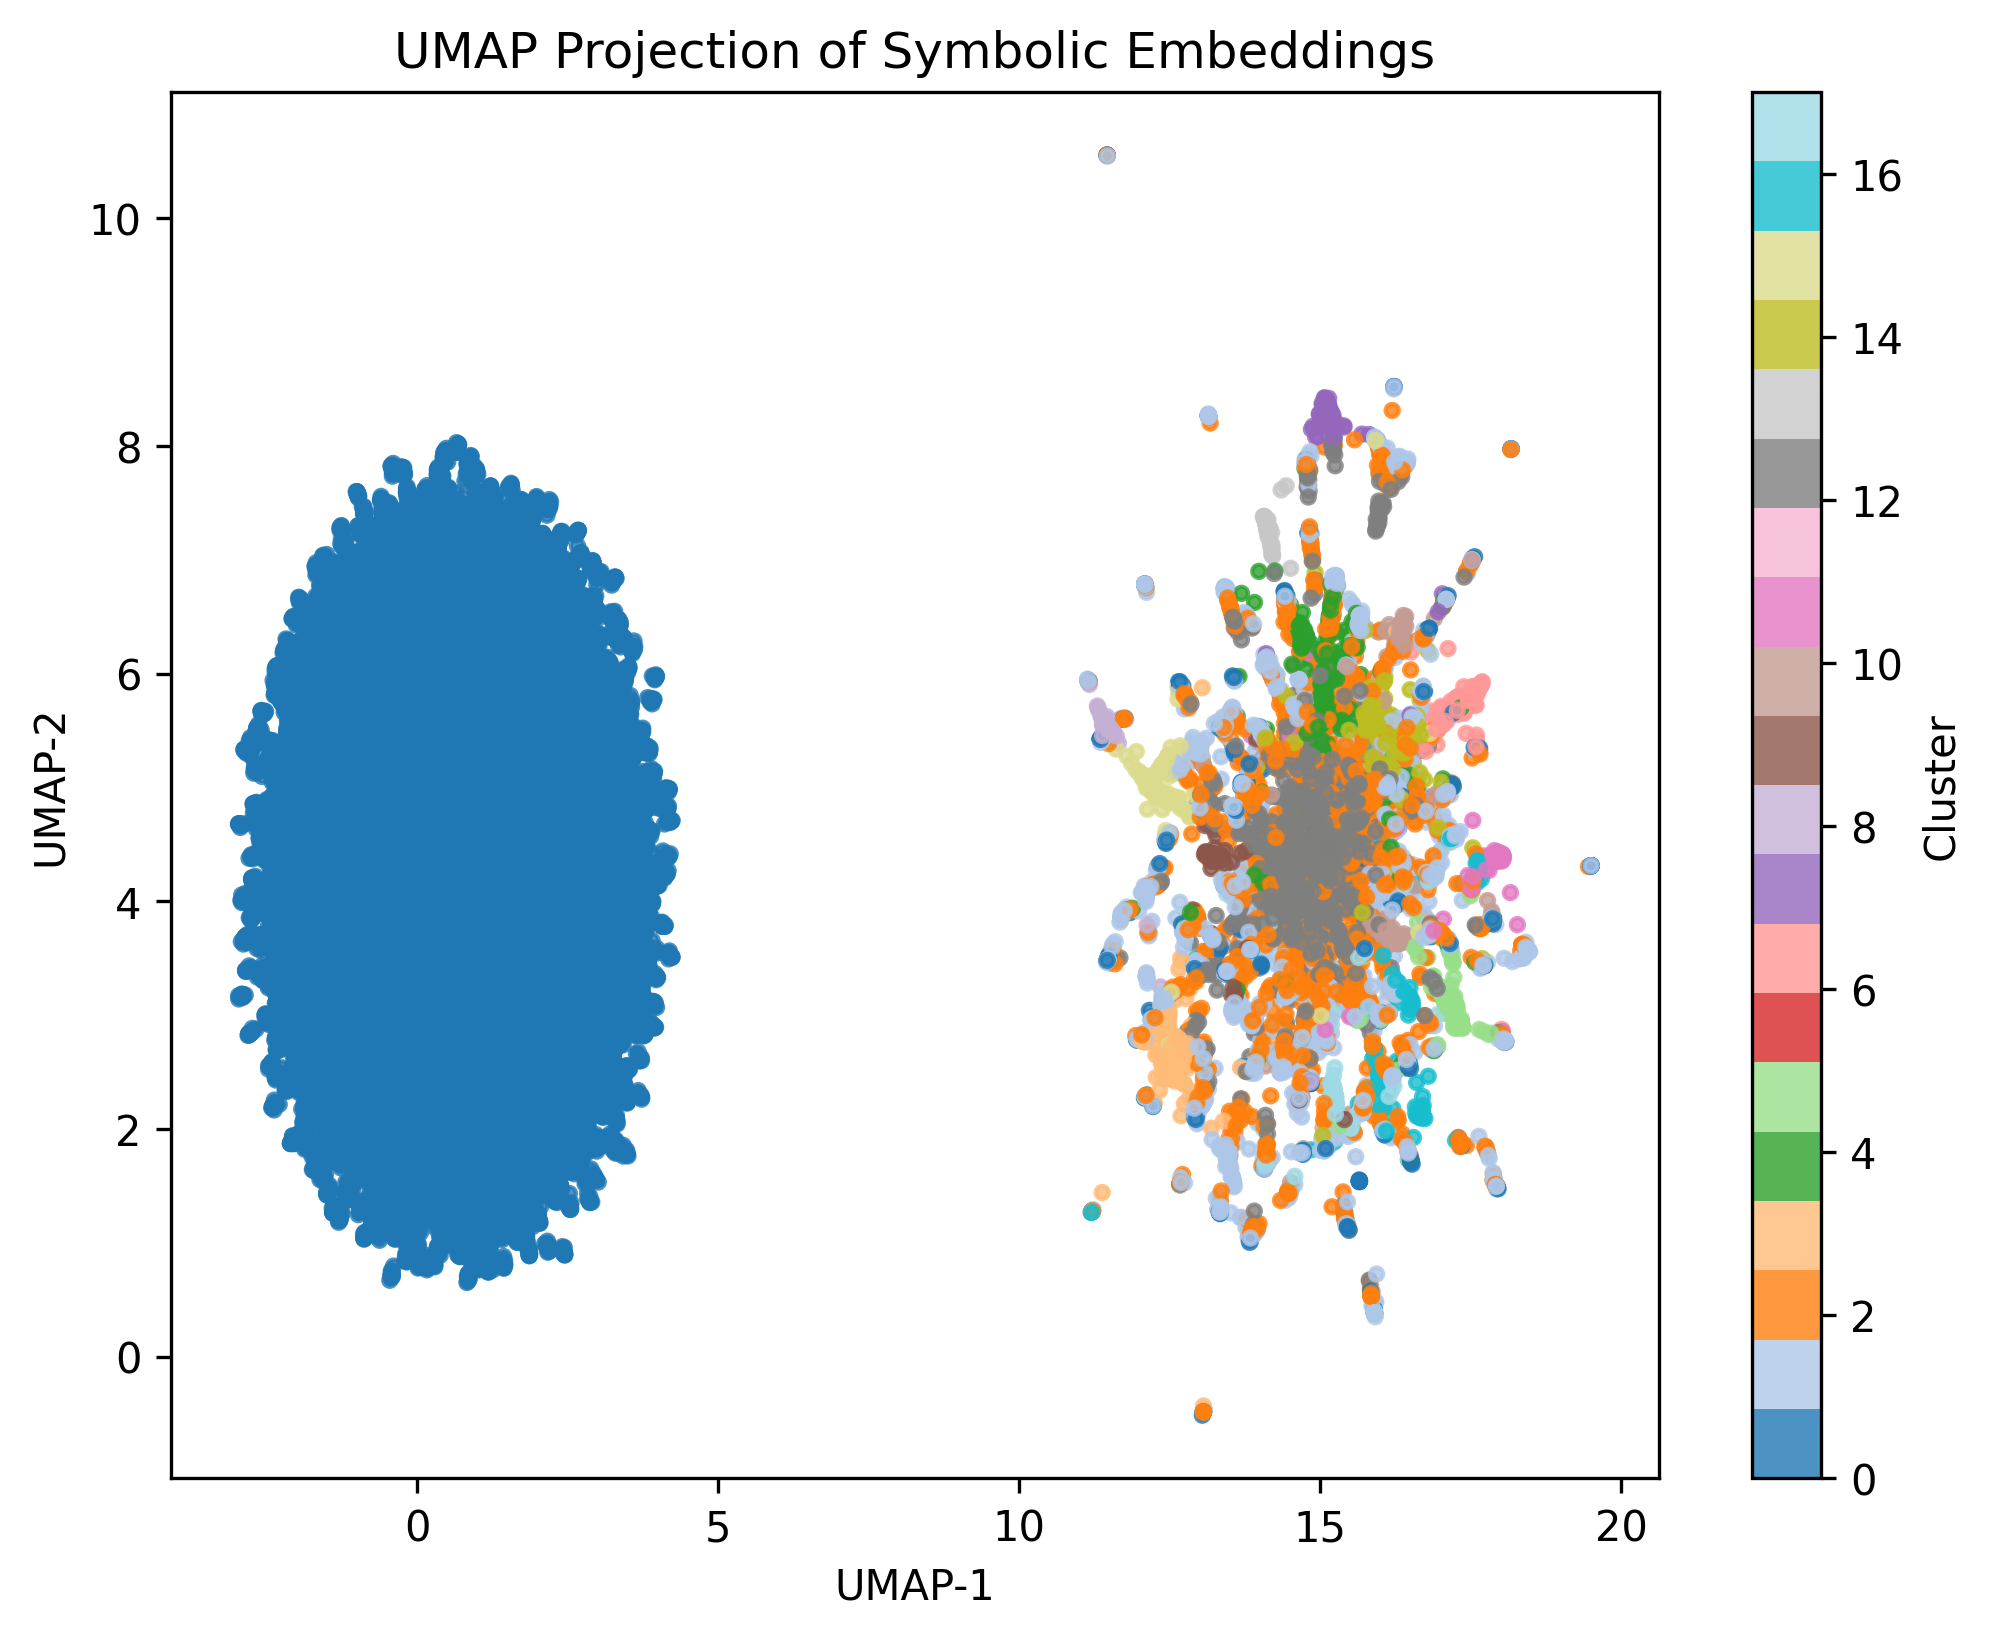
\includegraphics[width=\linewidth]{umap_projection.png}
\caption{\textbf{UMAP embeddings with density-based clustering.} Points represent node2vec embeddings projected to two dimensions; colours indicate HDBSCAN cluster labels. Insets (not shown) report soft-membership probabilities and outlier scores. Silhouette coefficients and cluster persistence statistics are provided in the Supplementary Information.}
\label{fig:umap}
\end{figure}

\subsection*{Entropic--geometric atlas of regimes}
Each network state is summarised by
\begin{equation}
\mathbf{m}=\big(H_{\mathrm{rate}}(P),\ \overline{\kappa}_{\mathrm{OR}},\ E_{\mathrm{glob}},\ C,\ Q,\ \mathrm{Gini}(\deg),\ \overline{c}_{\mathrm{eig}}\big),
\end{equation}
where $H_{\mathrm{rate}}$ is the entropy rate of $P$, $\overline{\kappa}_{\mathrm{OR}}$ the mean Ollivier--Ricci curvature over edges, $E_{\mathrm{glob}}$ global efficiency, $C$ clustering coefficient, $Q$ modularity, $\mathrm{Gini}(\deg)$ inequality of the degree distribution, and $\overline{c}_{\mathrm{eig}}$ mean eigenvector centrality. In practice, $(H_{\mathrm{rate}},\overline{\kappa}_{\mathrm{OR}})$ already provide a compact, interpretable \emph{entropic--geometric atlas}.

\begin{figure}[htbp]\centering
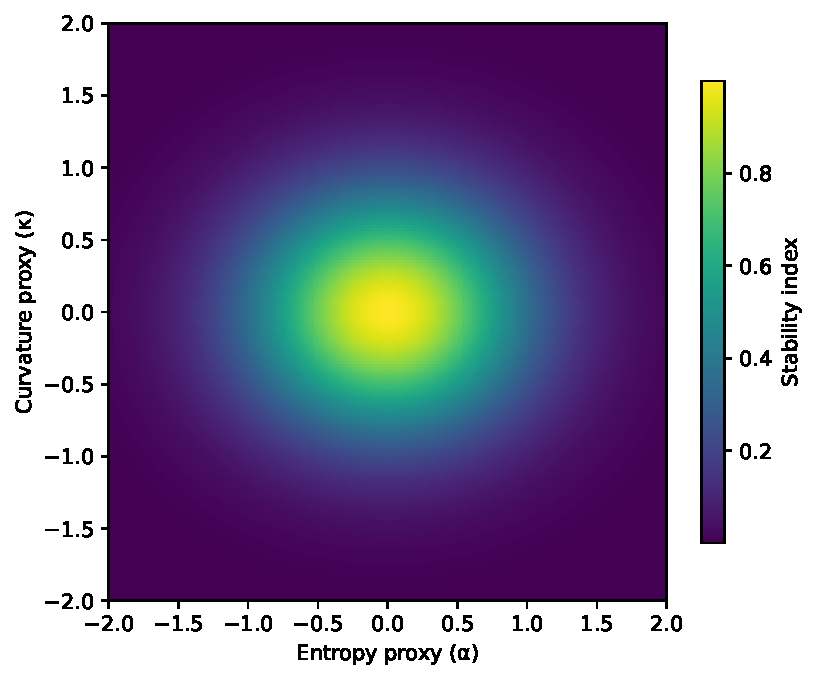
\includegraphics[width=\linewidth]{Fig_symbolic_heatmap.pdf}
\caption{\textbf{Entropy--curvature atlas of symbolic regimes.} Each point represents a network state positioned by its entropy rate ($H_{\mathrm{rate}}$, x-axis) and mean Ollivier--Ricci curvature ($\overline{\kappa}_{\mathrm{OR}}$, y-axis). Colours indicate canonical regimes. Kernel density estimates (marginals) reveal separable basins, illustrating complementary sensitivity of entropy and curvature to different perturbations.}
\label{fig:heatmap}
\end{figure}

\subsection*{Translational mapping: from simulations to regenerative contexts}
Regime signatures are mapped to translational contexts (Fig.~\ref{fig:map}): focal tract disruption (stroke/trauma) displays selective-disconnection patterns; diffuse degradation (neurodegeneration) approaches collapse; rehabilitation or neuroprosthetic integration pulls trajectories toward integration.

\begin{figure}[htbp]\centering
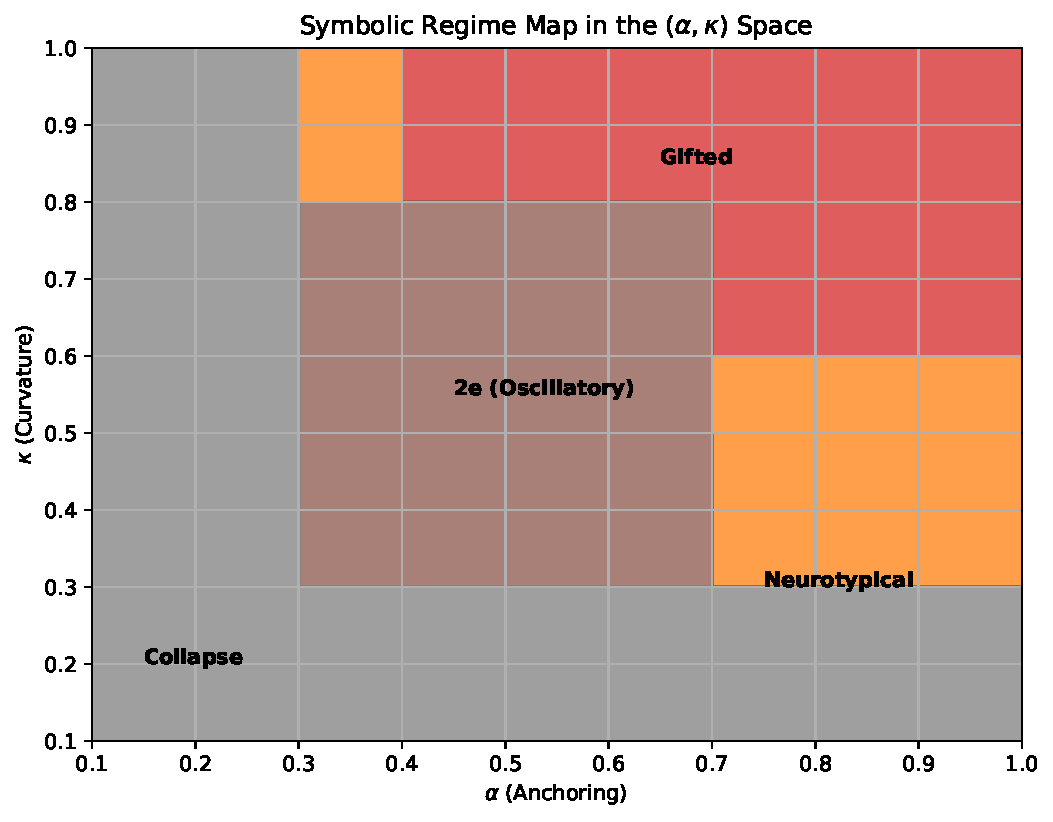
\includegraphics[width=\linewidth]{Fig_symbolic_regimes_map.pdf}
\caption{\textbf{Symbolic regime mapping and translational scenarios.} Diagram linking entropy--curvature patterns to neurobiological contexts. Arrows indicate hypothetical recovery pathways within the symbolic manifold; icons represent measurement modalities (e.g., neuroimaging, cognitive tasks).}
\label{fig:map}
\end{figure}

\subsection*{Temporal dynamics: collapse and recovery}
Figure~\ref{fig:collapse} shows a representative collapse--recovery trajectory under a perturbation onset (dashed line) affecting curvature and efficiency, with concurrent changes in effective activation breadth and an entropy-related measure.

\begin{figure}[htbp]\centering
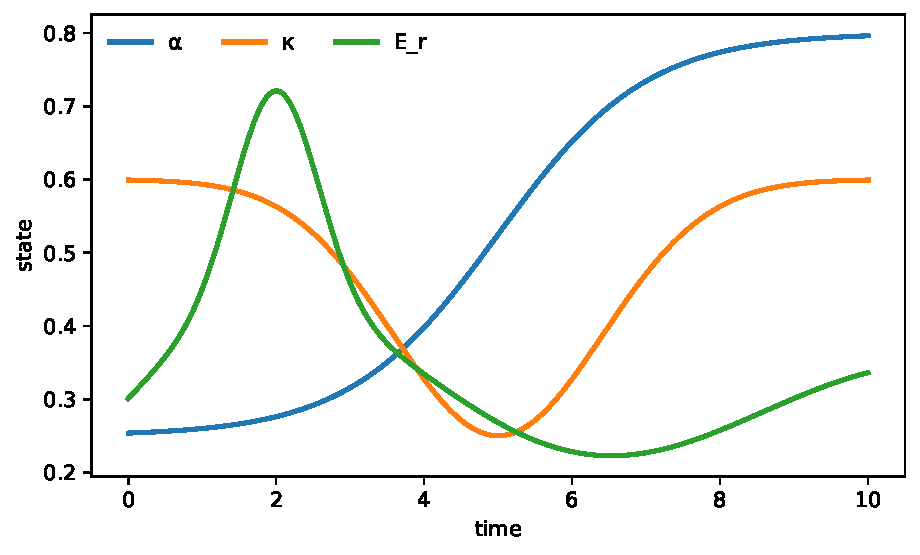
\includegraphics[width=\linewidth]{Fig_collapse_recovery.pdf}
\caption{\textbf{Collapse and recovery under perturbation.} Simulated time series of state variables showing the effect of a perturbation on curvature ($\kappa$), effective activation breadth ($\alpha$), and an entropy-related measure ($E_r$). Vertical dashed line: perturbation onset.}
\label{fig:collapse}
\end{figure}

\section*{Discussion}
We introduced a symbolic--semantic framework that integrates graph topology, entropy-controlled dynamics and discrete curvature into a low-dimensional manifold where cognitive regimes become separable and interpretable. On SWOW-EN, distinct perturbational profiles---integrated, hyper-associative, selective disconnection and collapse---yield non-redundant shifts in entropy rate and curvature, with consistent geometry in embedded space. We emphasise that these regime signatures are \emph{candidate} computational markers, not clinical endpoints; they are designed to be aligned with independent measurements in future work.

Entropy rate ($H_{\mathrm{rate}}$) proxies the breadth of symbolic exploration; mean Ollivier--Ricci curvature ($\overline{\kappa}_{\mathrm{OR}}$) captures local geometric coherence and bridge sensitivity. The $(H_{\mathrm{rate}},\overline{\kappa}_{\mathrm{OR}})$ plane thus constitutes an \emph{entropic--geometric atlas} in which regime trajectories are naturally expressed---e.g., targeted disconnection depresses curvature more than entropy, whereas indiscriminate noise inflates entropy while eroding cluster coherence.

Although the present study uses simulated regimes, the atlas offers a disciplined pathway for longitudinal alignment with behavioural measures (e.g., verbal fluency, lexical access latencies) and neuroimaging (EEG/fMRI/DTI). Hypothesis-generating examples include: focal tract disruption mapping to selective-disconnection signatures; diffuse degradation mapping to collapse; and rehabilitation/neuroprosthetic adaptation pulling trajectories towards integration. We refrain from clinical inference here; the intent is a stable computational coordinate system for future studies.

Methodologically, the pipeline is end-to-end, version-pinned and openly archived, with intermediate artefacts (metrics, embeddings, labels) saved for reuse. Stability is assessed under seed and hyperparameter variation, and under bootstrap perturbations of nodes/edges. Limitations include the use of population-level semantic norms (not subject-specific), reliance on simulated perturbations, modelling choices in curvature estimation, and dependence of manifold geometry on embedding/projection hyperparameters; we report robustness across reasonable grids.

\section*{Methods}

\subsection*{Data source and preprocessing}
We use SWOW-EN (Small World of Words; English) association norms \cite{DeDeyne2019}. Preprocessing: lowercase normalisation; removal of non-alphabetic tokens; optional lemmatisation for sensitivity checks; filtering rare edges by frequency threshold $\tau=3$ responses; retention of the giant weakly connected component. Edge weights $W_{ij}$ equal the empirical association frequency (or probability) from cue $i$ to associate $j$ after normalisation.

\subsection*{Graph construction and metrics}
We construct a directed weighted graph $G=(V,E,W)$. Degree (in/out), betweenness, closeness and eigenvector centrality are computed on $G$ (weighted, directed conventions as implemented in NetworkX). Global efficiency $E_{\mathrm{glob}}$ and clustering $C$ follow standard definitions \cite{Newman2010Networks,Latora2001PRL}. All network metrics were computed with NetworkX v2.8.8 \cite{NetworkX}, using directed and weighted conventions unless otherwise noted. Modularity $Q$ uses a directed extension with Louvain/Leiden (sensitivity analysis across seeds).

\subsection*{Entropic dynamics}
Define a $\beta$-controlled transition kernel $P(\beta)$ as above. The entropy rate of the induced Markov chain is
\begin{equation}
H_{\mathrm{rate}}(P) = - \sum_{i\in V} \pi_i \sum_{j\in V} P_{ij} \log P_{ij},
\end{equation}
where $\pi$ is the stationary distribution of $P$. We sweep $\beta$ on a grid ($\beta\in\{0.5,0.8,1.0,1.2,1.5,2.0\}$) and, for each $\beta$, apply controlled perturbations to $W$ to instantiate regimes: hyper-association (broadening of weak edges), selective disconnection (targeted removal of bridges/cut-sets), and fragmentation (random edge percolation).

\subsection*{Discrete curvature}
We compute Ollivier--Ricci curvature $\kappa_{\mathrm{OR}}(i,j)$ using one-step neighbour measures with $\alpha=0.5$ anchoring, i.e. $\mu_x=\alpha\delta_x+(1-\alpha)\,$Uniform$(\mathcal{N}(x))$, and
\begin{equation}
\kappa_{\mathrm{OR}}(i,j) = 1 - \frac{W_1(\mu_i,\mu_j)}{d(i,j)},
\end{equation}
where $W_1$ is a 1-Wasserstein distance and $d$ a graph distance \cite{Ollivier2009,Forman2003}. We also compute Forman curvature on the undirected approximation as a sensitivity check.

\subsection*{Embedding and dimensionality reduction}
Node representations are learned with node2vec (dimension $d=128$; walk length $L=30$; window $=10$; walks/node $=10$; $p=1$, $q=0.5$, seed=42) \cite{Grover2016node2vec}. UMAP projects to 2D ($n_{\mathrm{neighbours}}=30$, \texttt{min\_dist}=0.1) for visualisation and clustering \cite{McInnes2018UMAP}. Robustness to hyperparameters and seeds is reported in the Supplementary Information.

\subsection*{Clustering}
HDBSCAN is applied in UMAP space to obtain robust clusters with soft memberships (\texttt{min\_cluster\_size}=50, \texttt{min\_samples}=10, metric='euclidean', cluster\_selection\_epsilon=0.0) \cite{Campello2015}. We report the number of clusters, outlier fraction, and stability under bootstrap resampling.

\subsection*{Use of large language models (LLMs)}
We document the use of a large language model (GPT-5 Thinking) to assist with code refactoring and editorial polishing. All analyses, code and text were verified by the authors, who take full responsibility for the content.

\section*{Data availability}
SWOW-EN English association norms are publicly available via the Small World of Words project (De Deyne \emph{et al.}, 2019, Behavior Research Methods, DOI: 10.3758/s13428-018-1115-7). Derived datasets (metrics, embeddings, entropy--curvature summaries, cluster labels) and all figure source data are archived on Zenodo: DOI 10.5281/zenodo.16783257.

\section*{Code availability}
The full pipeline (preprocessing, graph construction, entropic dynamics, curvature computation, embedding, projection, clustering, stability analysis) is available at \url{https://github.com/agourakis82/entropic-symbolic-society}, with an archived snapshot on Zenodo (DOI: 10.5281/zenodo.16783257). Exact package versions and environments are pinned.

\section*{Acknowledgements}
[Insert funding, institutional support, and computational resources.]

\section*{Author contributions}
D.A. conceived the study and designed the computational framework. D.C.A., R.R.A., M.S.M., and M.G. contributed to theoretical framing, clinical context integration, and manuscript revision. All authors approved the final version.

\section*{Competing interests}
The authors declare no competing interests.

\section*{Supplementary Information}
Supplementary Information is provided as a single PDF file named \emph{Supplementary\_Information.pdf}, containing: (i) Mathematical Notes (definitions; lemma; proof sketch); (ii) Glossary and Table of Symbols; (iii) additional figures S1--S5 (ablation, null-model comparisons, curvature sensitivity, trajectories); (iv) source data tables for all main and supplementary figures.

\bibliography{refs}

\end{document}
